\section{Hyperbolic Functions}{}{}\label{sec:hyperbolic functions}

The \textbf{hyperbolic functions} are a set of functions that have many applications to mathematics, physics, and engineering. Among many other applications, they are used to describe the formation of satellite rings around planets, to describe the shape of a rope hanging from two points, and have application to the theory of special relativity. This section defines the hyperbolic functions and describes many of their properties, especially their usefulness to calculus.

These functions are sometimes referred to as the ``hyperbolic trigonometric functions'' as there are many, many connections between them and the standard trigonometric functions. Figure \ref{fig:geometric def trigh} demonstrates one such connection. Just as cosine and sine are used to define points on the circle defined by $x^2+y^2=1$, the functions \textbf{hyperbolic cosine} and \textbf{hyperbolic sine} are used to define points on the hyperbola $x^2-y^2=1$. This is a bit surprising given our initial definitions.

\begin{definition}{Hyperbolic Functions}{Hyperbolic Sine and Cosine}
\label{def:hyperbolic_functions}
%The \dfont{hyperbolic cosine} is the function
%$$\cosh x ={e^x +e^{-x }\over2},$$
%and the \dfont{hyperbolic sine} is the function
%$$\sinh x ={e^x -e^{-x}\over 2}.$$
\begin{minipage}{.5\textwidth}
\begin{enumerate}
\item		$\ds \cosh x = \frac{e^x+e^{-x}}2$\index{hyperbolic function!definition}
\item		$\ds \sinh x = \frac{e^x-e^{-x}}2$
\item		$\ds \tanh x = \frac{\sinh x}{\cosh x}$
\end{enumerate}
\end{minipage}
\begin{minipage}{.5\textwidth}
\begin{enumerate}\addtocounter{enumi}{3}
\item		$\ds \sech x = \frac{1}{\cosh x}$
\item		$\ds \csch x = \frac{1}{\sinh x}$
\item		$\ds \coth x = \frac{\cosh x}{\sinh x}$
\end{enumerate}
\end{minipage}
\end{definition}

These hyperbolic functions are graphed in Figure \ref{fig:hyperbolic}. In the graphs of $\cosh x$ and $\sinh x$, graphs of $e^x/2$ and $e^{-x}/2$ are included with dashed lines. As $x$ gets ``large,'' $\cosh x$ and $\sinh x$ each act like $e^x/2$; when $x$ is a large negative number, $\cosh x$ acts like $e^{-x}/2$ whereas $\sinh x$ acts like $-e^{-x}/2$.

Notice the domains of $\tanh x$ and $\sech x$ are $(-\infty,\infty)$, whereas both $\coth x$ and $\csch x$ have vertical asymptotes at $x=0$. Also note the ranges of these functions, especially $\tanh x$: as $x\to\infty$, both $\sinh x$ and $\cosh x$ approach $e^{-x}/2$, hence $\tanh x$ approaches $1$.

%It is no coincidence that these functions share a name similar to the trigonometric functions. 
The following example explores some of the properties of these functions that bear remarkable resemblance to the properties of their trigonometric counterparts.\\

{\textbf{Pronunciation Note:} \par 
``cosh'' rhymes with ``gosh,'' \par ``sinh'' rhymes with ``pinch,'' or alternatively is pronounced``shine" and \par ``tanh'' rhymes with ``ranch.'', or alternatively is pronounced``tank"}

Notice that $\cosh$ is even (that is, $\cosh(-x)=\cosh(x)$)
while $\sinh$ is odd ($\sinh(-x)=-\sinh(x)$), and
$\ds\cosh x + \sinh x = e^x$. Also, for all $x$,
$\cosh x >0$, while $\sinh x=0$ if and only if $\ds e^x -e^{-x }=0$,
which is true precisely when $x=0$.

\begin{theorem}{Range of Hyperbolic Cosine}{Range of Hyperbolic Cosine}
The range of $\cosh x$ is $[1,\infty)$.
\end{theorem}

\begin{proof}
Let $y= \cosh x$. We solve for $x$:
\begin{eqnarray*}
y&=&{e^x +e^{-x }\over 2}\cr
2y &=& e^x + e^{-x }\cr
2ye^x &=& e^{2x} + 1\cr
 0 &=& e^{2x}-2ye^x +1\cr
 e^{x} &=& {2y \pm \sqrt{4y^2 -4}\over 2}\cr
 e^{x} &=& y\pm \sqrt{y^2 -1}
\end{eqnarray*}
From the last equation, we see $\ds y^2 \geq 1$, and since
$y\geq 0$, it follows that $y\geq 1$.

Now suppose $y\geq 1$, so $\ds y\pm \sqrt{y^2 -1}>0$. Then
$\ds x = \ln(y\pm \sqrt{y^2 -1})$ is a real number, and 
$y =\cosh x$, so $y$ is in the range of $\cosh(x)$.
\end{proof}

%\begin{definition}{Hyperbolic Functions}{Hyperbolic Functions}
%We can also define hyperbolic functions for the other trigonometric functions as you would expect:
%$$\tanh x=\frac{\sinh x}{\cosh x}\qquad \csch x=\frac{1}{\sinh x}\qquad \sech x=\frac{1}{\cosh x}\qquad \coth x=\frac{1}{\tanh x}$$
%\end{definition}

The graphs can be generated based on our knowledge of the exponential function.  

%The graph of $\sinh x$ is shown below:
%$$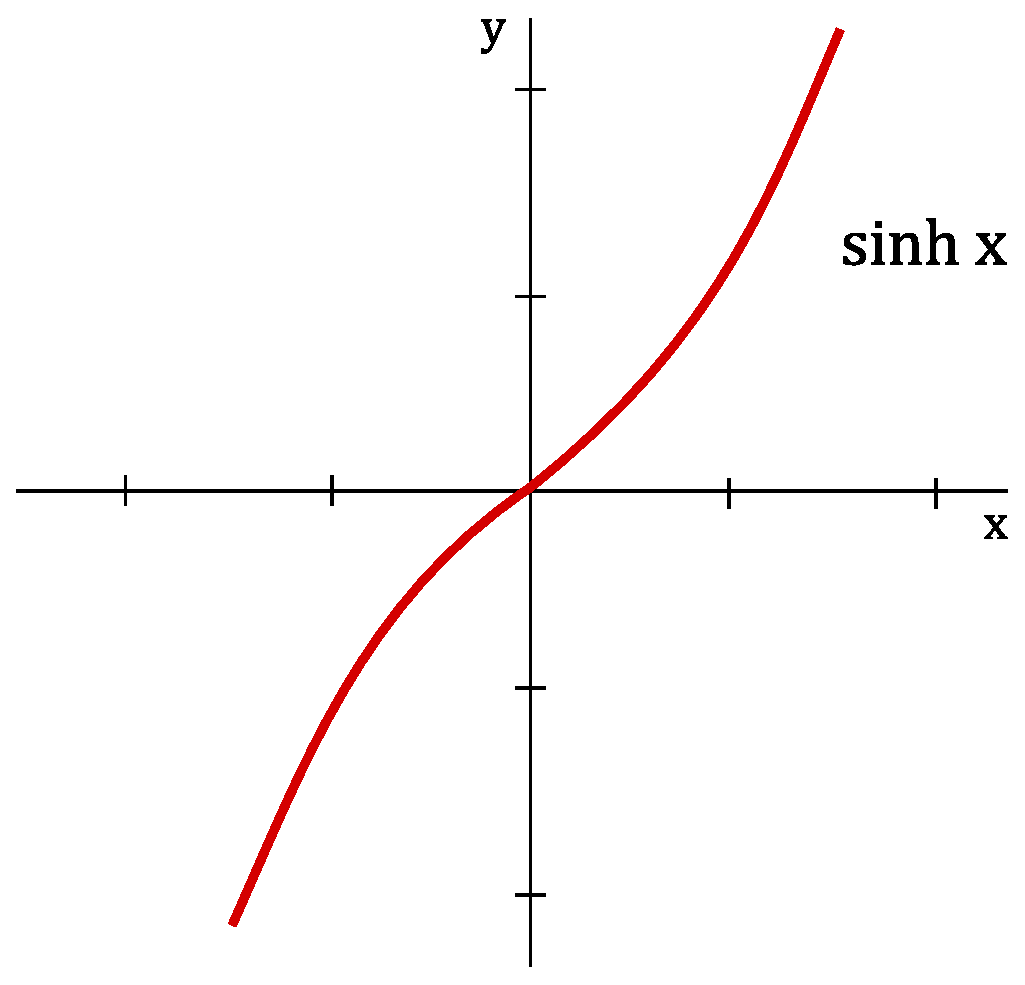
\includegraphics[width=2.5in]{images2/sinh}$$
%The graph of $\cosh x$ is shown below:
%$$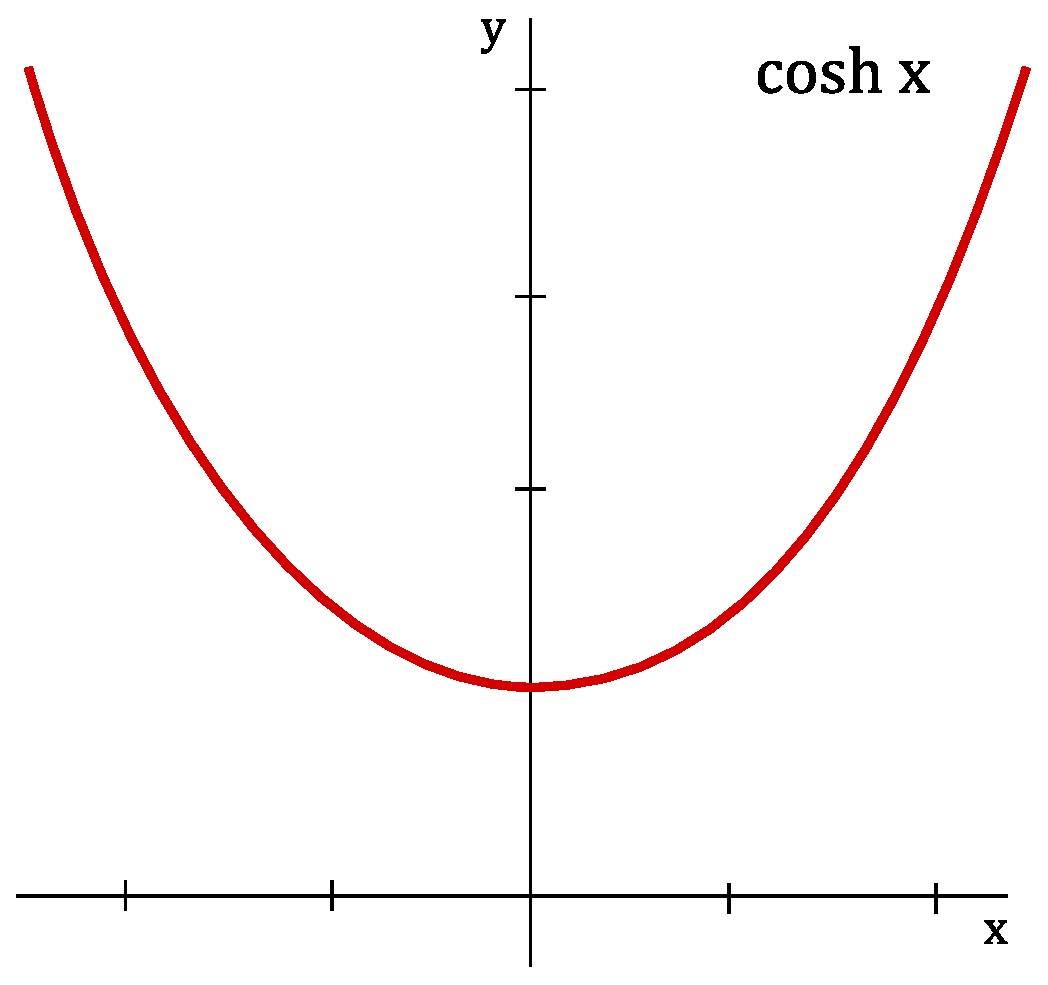
\includegraphics[width=2.5in]{images2/cosh}$$

\begin{figure}
\begin{subfigure}{.5\textwidth}
  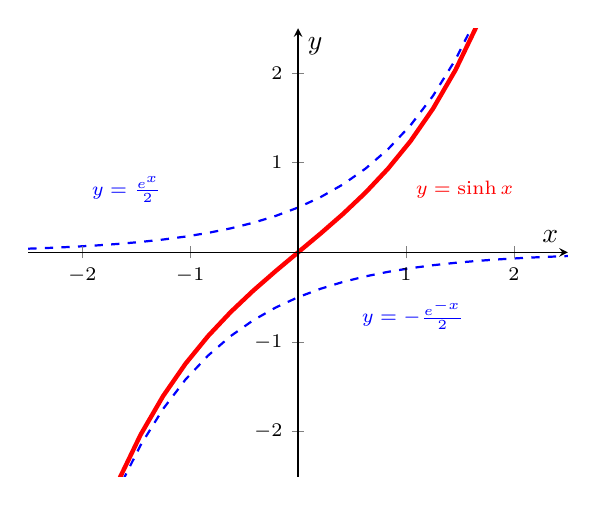
\begin{tikzpicture}
\begin{axis}[tick label style={font=\scriptsize},
    xmin=-2.5, xmax=2.5,
    ymin=-2.5, ymax=2.5,
    axis lines=center,
    axis on top=true,
    domain=-2.5:2.5,
    ylabel=$y$,
    xlabel=$x$,
    ]

    \addplot [mark=none,draw=red,ultra thick] {sinh(\x)};
    \addplot [mark=none,draw=blue,dashed, thick] {(1/2)*exp(\x)};
    \addplot [mark=none,draw=blue, dashed,thick] {(-1/2)*exp(-\x)};
    \node [right, red] at (axis cs: 1,0.7) {\scriptsize $y = \sinh x$};
    \node [right, blue] at (axis cs: -2,0.7) {\scriptsize $\ds y = \frac{e^x}{2}$};
    \node [right, blue] at (axis cs: 0.5,-0.7) {\scriptsize $\ds y = -\frac{e^{-x}}{2}$};

    %% Add the asymptotes
   %\draw [blue, dotted, thick] (axis cs:-2.5,-1)-- (axis cs:0,-1);
  %  \draw [blue, dotted, thick] (axis cs:+2.5,+1)-- (axis cs:0,+1);
\end{axis}
\end{tikzpicture}
\end{subfigure}
\begin{subfigure}{.5\textwidth}
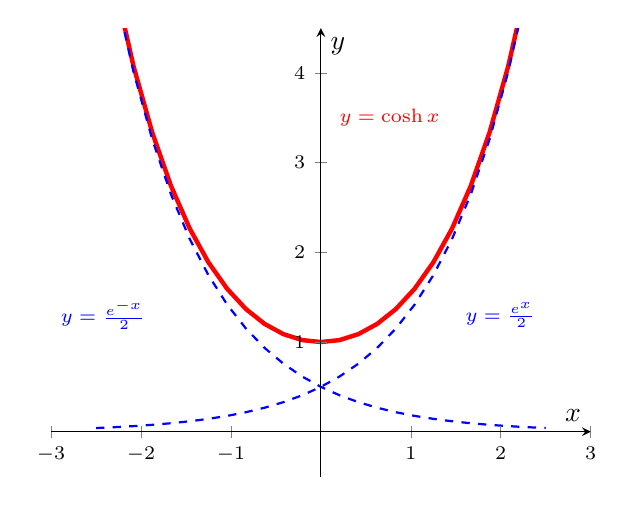
\begin{tikzpicture}
\begin{axis}[tick label style={font=\scriptsize},
    xmin=-3, xmax=3,
    ymin=-0.5, ymax=4.5,
    axis lines=center,
    axis on top=true,
    domain=-2.5:2.5,
    ylabel=$y$,
    xlabel=$x$,
    ]

    \addplot [mark=none,draw=red,ultra thick] {cosh(\x)};
    \addplot [mark=none,draw=blue,dashed, thick] {(1/2)*exp(\x)};
    \addplot [mark=none,draw=blue,dashed, thick] {(1/2)*exp(-\x)};
    \node [right, red] at (axis cs: 0.1,3.5) {\scriptsize $y = \cosh x$};
    \node [right, blue] at (axis cs: 1.5,1.3) {\scriptsize $\ds y = \frac{e^x}{2}$};
    \node [right, blue] at (axis cs: -3,1.3) {\scriptsize $\ds y = \frac{e^{-x}}{2}$};

    %% Add the asymptotes
    %\draw [blue, dotted, thick] (axis cs:-2.5,-1)-- (axis cs:0,-1);
    %\draw [blue, dotted, thick] (axis cs:+2.5,+1)-- (axis cs:0,+1);
\end{axis}
\end{tikzpicture}
\end{subfigure}
\begin{subfigure}{.5\textwidth}
\begin{tikzpicture}
\begin{axis}[width=\textwidth,%
tick label style={font=\scriptsize},axis y line=middle,axis x line=middle,name=myplot,axis on top,%
			%x=.37\marginparwidth,
			%y=.37\marginparwidth,
%			xtick=\empty,% 
%			extra x ticks={.5,3},
%			extra x tick labels={$a$,$b$},
			ytick={-2,2},
%			yticklabels={$-0.002$,$0.002$,$0.004$},
			%minor y tick num=1,
%			extra y ticks={0.001},%
%			minor x tick num=4,
			ymin=-3.5,ymax=3.5,%
			xmin=-3.5,xmax=3.5,%
			scaled ticks=false
]

\addplot [{\colorone},thick,smooth] coordinates {(-3.,-0.995)(-2.9,-0.994)(-2.8,-0.993)(-2.7,-0.991)(-2.6,-0.989)(-2.5,-0.987)(-2.4,-0.984)(-2.3,-0.98)(-2.2,-0.976)(-2.1,-0.97)(-2.,-0.964)(-1.9,-0.956)(-1.8,-0.947)(-1.7,-0.935)(-1.6,-0.922)(-1.5,-0.905)(-1.4,-0.885)(-1.3,-0.862)(-1.2,-0.834)(-1.1,-0.8)(-1.,-0.762)(-0.9,-0.716)(-0.8,-0.664)(-0.7,-0.604)(-0.6,-0.537)(-0.5,-0.462)(-0.4,-0.38)(-0.3,-0.291)(-0.2,-0.197)(-0.1,-0.0997)(0,0)(0.1,0.0997)(0.2,0.197)(0.3,0.291)(0.4,0.38)(0.5,0.462)(0.6,0.537)(0.7,0.604)(0.8,0.664)(0.9,0.716)(1.,0.762)(1.1,0.8)(1.2,0.834)(1.3,0.862)(1.4,0.885)(1.5,0.905)(1.6,0.922)(1.7,0.935)(1.8,0.947)(1.9,0.956)(2.,0.964)(2.1,0.97)(2.2,0.976)(2.3,0.98)(2.4,0.984)(2.5,0.987)(2.6,0.989)(2.7,0.991)(2.8,0.993)(2.9,0.994)(3.,0.995)};

\draw (axis cs:1.7,-1.5) node {\scriptsize $f(x)=\tanh x$};
\draw (axis cs:2.2,2) node {\scriptsize $f(x)=\coth x$};
\draw [->,>=stealth] (axis cs:1,-1) -- (axis cs:.6,.45);


\addplot [{\colortwo},smooth,thick] coordinates {(-3.,-1.)(-2.9,-1.01)(-2.8,-1.01)(-2.7,-1.01)(-2.6,-1.01)(-2.5,-1.01)(-2.4,-1.02)(-2.3,-1.02)(-2.2,-1.02)(-2.1,-1.03)(-2.,-1.04)(-1.9,-1.05)(-1.8,-1.06)(-1.7,-1.07)(-1.6,-1.08)(-1.5,-1.1)(-1.4,-1.13)(-1.3,-1.16)(-1.2,-1.2)(-1.1,-1.25)(-1.,-1.31)(-0.9,-1.4)(-0.8,-1.51)(-0.7,-1.65)(-0.6,-1.86)(-0.5,-2.16)(-0.4,-2.63)(-0.3,-3.43)(-0.2,-5.07)(-0.1,-10.)};

\addplot [{\colortwo},smooth,thick] coordinates {(0.1,10.)(0.2,5.07)(0.3,3.43)(0.4,2.63)(0.5,2.16)(0.6,1.86)(0.7,1.65)(0.8,1.51)(0.9,1.4)(1.,1.31)(1.1,1.25)(1.2,1.2)(1.3,1.16)(1.4,1.13)(1.5,1.1)(1.6,1.08)(1.7,1.07)(1.8,1.06)(1.9,1.05)(2.,1.04)(2.1,1.03)(2.2,1.02)(2.3,1.02)(2.4,1.02)(2.5,1.01)(2.6,1.01)(2.7,1.01)(2.8,1.01)(2.9,1.01)(3.,1.)};
%\draw (axis cs:2.4,-0.002) node {\scriptsize $f(x)$};
\draw [loosely dashed] (axis cs:-3,1) -- (axis cs:3,1);
\draw [loosely dashed] (axis cs:-3,-1) -- (axis cs:3,-1);

\end{axis}

\node [right] at (myplot.right of origin) {\scriptsize $x$};
\node [above] at (myplot.above origin) {\scriptsize $y$};
\end{tikzpicture}
\end{subfigure}
\begin{subfigure}{.5\textwidth}
\begin{tikzpicture}
\begin{axis}[width=\textwidth,%
tick label style={font=\scriptsize},axis y line=middle,axis x line=middle,name=myplot,axis on top,%
			%x=.37\marginparwidth,
			%y=.37\marginparwidth,
%			xtick=\empty,% 
%			extra x ticks={.5,3},
%			extra x tick labels={$a$,$b$},
			ytick={-3,-2,-1,1,2,3},
%			yticklabels={$-0.002$,$0.002$,$0.004$},
			%minor y tick num=1,
%			extra y ticks={0.001},%
%			minor x tick num=4,
			ymin=-3.5,ymax=3.5,%
			xmin=-3.5,xmax=3.5,%
			scaled ticks=false
]

\addplot [{\colorone},thick,smooth] coordinates {(-3.,0.0993)(-2.9,0.11)(-2.8,0.121)(-2.7,0.134)(-2.6,0.148)(-2.5,0.163)(-2.4,0.18)(-2.3,0.199)(-2.2,0.219)(-2.1,0.241)(-2.,0.266)(-1.9,0.293)(-1.8,0.322)(-1.7,0.354)(-1.6,0.388)(-1.5,0.425)(-1.4,0.465)(-1.3,0.507)(-1.2,0.552)(-1.1,0.599)(-1.,0.648)(-0.9,0.698)(-0.8,0.748)(-0.7,0.797)(-0.6,0.844)(-0.5,0.887)(-0.4,0.925)(-0.3,0.957)(-0.2,0.98)(-0.1,0.995)(0,1.)(0.1,0.995)(0.2,0.98)(0.3,0.957)(0.4,0.925)(0.5,0.887)(0.6,0.844)(0.7,0.797)(0.8,0.748)(0.9,0.698)(1.,0.648)(1.1,0.599)(1.2,0.552)(1.3,0.507)(1.4,0.465)(1.5,0.425)(1.6,0.388)(1.7,0.354)(1.8,0.322)(1.9,0.293)(2.,0.266)(2.1,0.241)(2.2,0.219)(2.3,0.199)(2.4,0.18)(2.5,0.163)(2.6,0.148)(2.7,0.134)(2.8,0.121)(2.9,0.11)(3.,0.0993)};

\draw (axis cs:-2,1.5) node {\scriptsize $f(x)=\sech x$};
\draw (axis cs:2.2,2) node {\scriptsize $f(x)=\csch x$};
%\draw [->,>=latex] (axis cs:1,-1) -- (axis cs:.6,.45);


\addplot [{\colortwo},smooth,thick] coordinates {(-3.,-0.0998)(-2.9,-0.11)(-2.8,-0.122)(-2.7,-0.135)(-2.6,-0.149)(-2.5,-0.165)(-2.4,-0.183)(-2.3,-0.203)(-2.2,-0.224)(-2.1,-0.249)(-2.,-0.276)(-1.9,-0.306)(-1.8,-0.34)(-1.7,-0.378)(-1.6,-0.421)(-1.5,-0.47)(-1.4,-0.525)(-1.3,-0.589)(-1.2,-0.662)(-1.1,-0.749)(-1.,-0.851)(-0.9,-0.974)(-0.8,-1.13)(-0.7,-1.32)(-0.6,-1.57)(-0.5,-1.92)(-0.4,-2.43)(-0.3,-3.28)(-0.2,-4.97)(-0.1,-9.98)};

\addplot [{\colortwo},smooth,thick] coordinates {(0.1,9.98)(0.2,4.97)(0.3,3.28)(0.4,2.43)(0.5,1.92)(0.6,1.57)(0.7,1.32)(0.8,1.13)(0.9,0.974)(1.,0.851)(1.1,0.749)(1.2,0.662)(1.3,0.589)(1.4,0.525)(1.5,0.47)(1.6,0.421)(1.7,0.378)(1.8,0.34)(1.9,0.306)(2.,0.276)(2.1,0.249)(2.2,0.224)(2.3,0.203)(2.4,0.183)(2.5,0.165)(2.6,0.149)(2.7,0.135)(2.8,0.122)(2.9,0.11)(3.,0.0998)};
%\draw (axis cs:2.4,-0.002) node {\scriptsize $f(x)$};
\end{axis}

\node [right] at (myplot.right of origin) {\scriptsize $x$};
\node [above] at (myplot.above origin) {\scriptsize $y$};
\end{tikzpicture}
\end{subfigure} 
\caption{Graphs of the Hyperbolic Functions\label{fig:hyperbolic}}
\end{figure}





Certainly the hyperbolic functions do not closely resemble the
trigonometric functions graphically. But they do have analogous
properties, beginning with the following identity.

\begin{theorem}{Hyperbolic Identity}{Hyperbolic Identity}
\label{hyp identity}
For all $x$ in $\R$, $\ds \cosh ^2 x -\sinh ^2 x = 1$.
\end{theorem}


\begin{proof}
The proof is a straightforward computation:
$$\cosh ^2 x -\sinh ^2 x =
 {(e^x +e^{-x} )^2\over 4} -{(e^x -e^{-x} )^2\over 4}=
 {e^{2x} + 2 + e^{-2x } - e^{2x } + 2 - e^{-2x}\over 4}=
 {4\over 4} = 1.
$$
\end{proof}

This immediately gives two additional identities:
$$1-\tanh^2 x =\sech^2 x\qquad\hbox{and}\qquad
\coth^2 x - 1  =\csch^2 x.$$

The identity of the theorem also helps to provide a geometric
motivation. Recall that the graph of $\ds x^2 -y^2 =1$ is a hyperbola
with asymptotes $x=\pm y$ whose $x$-intercepts are $\pm 1$. If
$(x,y)$ is a point on the right half of the hyperbola, and if
we let $x=\cosh \theta$, then
$\ds y=\pm\sqrt{x^2-1}=\pm\sqrt{\cosh^2x-1}=\pm\sinh \theta$. So for some
suitable $\theta$, $\cosh \theta$ and $\sinh \theta$ are the coordinates of a typical
point on the hyperbola. In fact, it turns out that $\theta$ is twice the
area shown in the first graph of  figure~\ref{fig:geometric def trigh}.  Even
this is analogous to trigonometry; $\cos \theta$ and $\sin \theta$ are the
coordinates of a typical point on the unit circle, and $\theta$ is twice
the area shown in the second graph of Figure~\ref{fig:geometric def
trigh}. 


\mtable{.7}{Using trigonometric functions to define points on a circle and hyperbolic functions to define points on a hyperbola. The area of the shaded regions are included in them. \label{fig:geometric def trigh}}{fig:hfcircle}{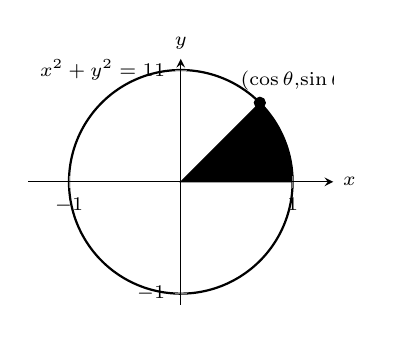
\begin{tikzpicture}
\begin{axis}[width=.45\textwidth,%
axis equal,
tick label style={font=\scriptsize},axis y line=middle,axis x line=middle,name=myplot,axis on top,%
			%x=.37\marginparwidth,
			%y=.37\marginparwidth,
			xtick={-1,1},% 
%			extra x ticks={.5,3},
%			extra x tick labels={$a$,$b$},
			ytick={-1,1},
			%minor y tick num=1,%extra y ticks={-5,-3,...,7},%
%			minor x tick num=4,
			ymin=-1.1,ymax=1.1,%
			xmin=-1.1,xmax=1.1%
]

\addplot [{\coloronefill},fill={\coloronefill},domain=0:45] ({cos(x)},{sin(x)}) -- (axis cs:0,0)--cycle;

\addplot [{\colorone},domain=0:360,thick,smooth,samples=100] ({cos(x)},{sin(x)});

\filldraw (axis cs:.707,.707) circle (2pt) node [shift={(13pt,8pt)}] {\scriptsize ($\cos \theta$,$\sin \theta$)};

\draw (axis cs:.6,.25) node {\scriptsize $\ds\frac{\theta}{2}$};
\draw (axis cs:-.75,1) node {\scriptsize $x^2+y^2=1$};

\end{axis}

\node [right] at (myplot.right of origin) {\scriptsize $x$};
\node [above] at (myplot.above origin) {\scriptsize $y$};
\end{tikzpicture}\hspace*{25pt}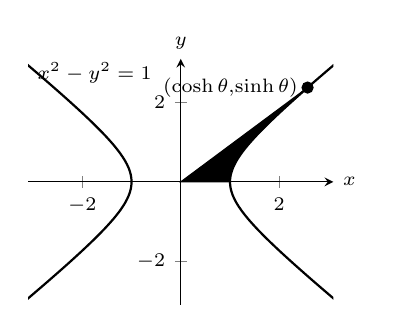
\begin{tikzpicture}
\begin{axis}[width=.45\textwidth,%
tick label style={font=\scriptsize},axis y line=middle,axis x line=middle,name=myplot,axis on top,%
			%x=.37\marginparwidth,
			%y=.37\marginparwidth,
%			xtick={.25,.5,.75,1},% 
%			extra x ticks={.5,3},
%			extra x tick labels={$a$,$b$},
%			ytick=\empty,
			%minor y tick num=1,%extra y ticks={-5,-3,...,7},%
%			minor x tick num=4,
			ymin=-3.1,ymax=3.1,%
			xmin=-3.1,xmax=3.1%
]

\addplot [{\coloronefill},fill={\coloronefill},domain=0:1.6] ({cosh(x)},{sinh(x)}) -- (axis cs:0,0)--cycle;

\addplot [{\colorone},domain=-2:2,thick,smooth] ({cosh(x)},{sinh(x)});
\addplot [{\colorone},domain=-2:2,thick,smooth] ({-cosh(x)},{sinh(x)});

\filldraw (axis cs:2.577,2.376) circle (2pt) node [left] {\scriptsize ($\cosh \theta$,$\sinh \theta$)};

\draw (axis cs:.73,.32) node {\scriptsize $\frac{\theta}{2}$};
\draw (axis cs:-1.75,2.75) node {\scriptsize $x^2-y^2=1$};

\end{axis}

\node [right] at (myplot.right of origin) {\scriptsize $x$};
\node [above] at (myplot.above origin) {\scriptsize $y$};
\end{tikzpicture}}


%\begin{figure}[!ht]
%$$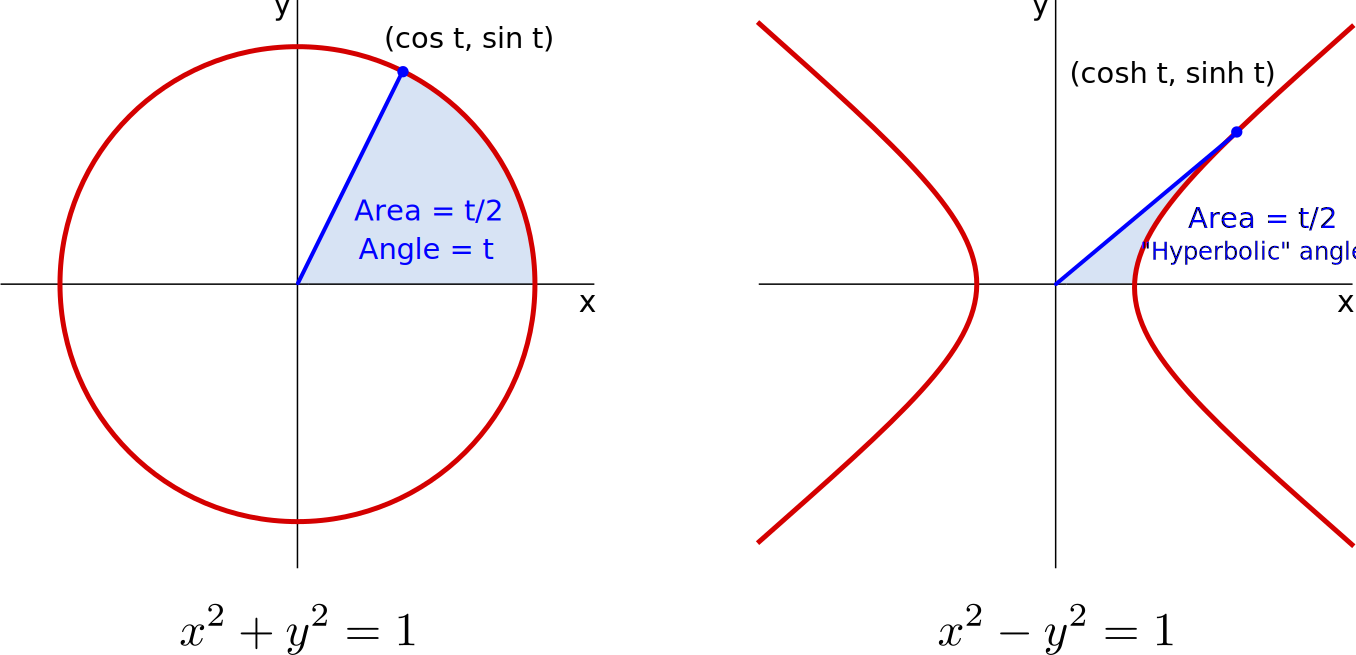
\includegraphics[width=5in]{images2/sinh-and-cosh-motivation}$$
%\caption{\label{fig:geometric def trigh}
%Geometric definitions. Here, $t$ is twice the shaded area in each figure.}
%\end{figure}

\begin{example}{Computing Hyperbolic Tangent}{Computing Hyperbolic Tangent}
 Use the definition of the hyperbolic functions to rewrite the following expressions.
\begin{enumerate}
%\item		$\cosh^2 x-\sinh^2x$
\item		$\tanh^2 x+\sech^2 x$
\item		$2\cosh x\sinh x$
\item		$\tanh(\ln 2)$.
\end{enumerate}
\end{example} 

\begin{solution}
\begin{enumerate}
%\item		%\vskip-\baselineskip%
%\hfill$\begin{aligned}[t]
% \cosh^2x-\sinh^2x &= \left(\frac{e^x+e^{-x}}2\right)^2 -\left(\frac{e^x-e^{-x}}2\right)^2\\
% 						&= \frac{e^{2x}+2e^xe^{-x} + e^{-2x}}4 - \frac{e^{2x}-2e^xe^{-x} + e^{-2x}}4\\
% 						&= \frac44=1.
%\end{aligned}$\hfill
%So $\cosh^2 x-\sinh^2x=1$.
\item $\begin{aligned}[t]
\tanh^2 x+\sech^2 x  =\frac{\sinh^2x}{\cosh^2 x} + \frac{1}{\cosh^2 x} 
					&= \frac{\sinh^2x+1}{\cosh^2 x}\qquad \text{\small Now use Theorem \ref{hyp identity}.}\\
					&= \frac{\cosh^2 x}{\cosh^2 x} = 1.\\
\end{aligned}$
 
So $\tanh^2 x+\sech^2 x=1$.
\item $\begin{aligned}[t]
	2\cosh x\sinh x &= 2\left(\frac{e^x+e^{-x}}2\right)\left(\frac{e^x-e^{-x}}2\right) \\
					&= 2 \cdot\frac{e^{2x} - e^{-2x}}4\\
					&= \frac{e^{2x} - e^{-2x}}2 = \sinh (2x).\\
			\end{aligned}$ 
			
Thus $2\cosh x\sinh x = \sinh (2x)$.
\item $\begin{aligned}[t]
	\tanh(\ln 2) & =\frac{\sinh(\ln 2)}{\cosh(\ln 2)}\\
	             & = \frac{\ds\frac{e^{\ln 2}-e^{-\ln 2}}{2}}{\ds\frac{e^{\ln 2}+e^{-\ln 2}}{2}}\\
	%= \frac{\ds\frac{e^{\ln 2}-e^{\ln(1/2)}}{2}}{\ds\frac{e^{\ln 2}+e^{\ln(1/2)}}{2}}
	&=  \frac{\ds\frac{2-(1/2)}{2}}{\ds\frac{2+(1/2)}{2}}
	 =\frac{2-(1/2)}{2+(1/2)}
	%=  \frac{3/2}{5/2}
	= \frac{3}{5}\\
			\end{aligned}$ 
			
Thus $\tanh(\ln 2) = \frac35$.
\end{enumerate}
\end{solution}

The following summarizes some of the important identities relating to hyperbolic functions. Each can be verified by referring back to Definition \ref{def:hyperbolic_functions}.

\textbf{Basic Identities}\par
\begin{enumerate}
\item $\cosh^2x-\sinh^2x=1$%
\index{hyperbolic function!identities}\index{hyperbolic function!derivatives}\index{hyperbolic function!integrals}\index{derivative!hyperbolic funct.}\index{integration!hyperbolic funct.}%
\item	$\tanh^2x+\sech^2x=1$
\item	$\coth^2x-\csch^2x = 1$
\item	$\cosh 2x=\cosh^2x+\sinh^2x$
\item	$\sinh 2x = 2\sinh x\cosh x$
\item	$\ds\cosh^2x = \frac{\cosh 2x+1}{2}$
\item $\ds \sinh^2x=\frac{\cosh 2x-1}{2}$
\end{enumerate}




%\figure
%\texonly
%\hbox to \hsize{\hfill
%\tikzpicture[domain=0:3,x=6mm,y=6mm,baseline=0]
%\draw (0,0) -- (3,0) ;
%\draw (0,-3) -- (0,3) ;
%\foreach \x in {1,2,3} \draw (\x,0) -- (\x,-2pt) node[anchor=north] {\eightpoint $\x$};
%\foreach \y in {-3,-2,-1,0,1,2,3} \draw (0,\y) -- (-2pt,\y) node[anchor=east]
%{\eightpoint $\y$};
%\node[anchor=west] at (2,1.3) {\ninepoint $(\cosh t,\sinh t)$};
%\global\advance\gpnum by 1
%\draw[color=black] plot[parametric,id=\the\gpnum,domain=-1:1] 
%function{1+2*t**2,2*t*sqrt(t**2+1)};
%\draw (0,0) -- (2,1.732); 
%\gpad
%\fill[opacity=0.5,fill=red!20] 
%(0,0) -- (1,0) 
%plot[parametric,id=\the\gpnum,domain=0:.707]
%function{1+2*t**2,2*t*sqrt(t**2+1);} -- (0,0);
%\node at  (2,1.732) {\fivepoint$\bullet$};
%\endtikzpicture
%\hskip2cm
%\tikzpicture[domain=-1.2:1.2,baseline=0]
%\draw (-1.2,0) -- (1.2,0) ;
%\draw (0,-1.2) -- (0,1.2) ;
%\foreach \x in {1} \draw (\x,0) -- (\x,-2pt) node[anchor=north west]
         %{\ninepoint $\x$};
%\node[anchor=south west] at (0.5,0.886) {\ninepoint $(\cos t,\sin t)$};
%\draw[color=black] (0,0) circle (1);
%\draw (0,0) -- (0.5,0.886); 
%\fill[opacity=0.5,fill=red!20] 
%(0,0) -- (1,0) arc (0:60:1) -- (0,0);
%\node[anchor=mid] at  (0.5,0.886) {\fivepoint$\bullet$};
%\endtikzpicture\hfill}
%\endtexonly
%\figrdef{fig:geometric def trigh}
%\htmlfigure{Transcendental-GeomDefs.html}
%\begincaption
%Geometric definitions of sin, cos, sinh, cosh: $t$ is twice the shaded
%area in each figure.
%\endcaption
%\endfigure

Since $\cosh x > 0$, $\sinh x$ is increasing and hence one-to-one, so
$\sinh x$ has an inverse, ${\rm arcsinh} x$. Also, $\sinh x > 0$ when
$x>0$, so $\cosh x$ is injective on $[0,\infty)$ and has a (partial)
inverse, ${\rm arccosh} x$. The other hyperbolic functions have inverses
as well, though ${\rm arcsech} x$ is only a partial inverse. 


%%%%%%%%%%%%%%%%%%%%%%%%%%%%%%%%%%%%%%%%%%%%
\Opensolutionfile{solutions}[ex]
\section*{Exercises for \ref{sec:hyperbolic functions}}

\begin{enumialphparenastyle}

%%%%%%%%%%

\begin{ex}
Verify the given identity using Definition \ref{def:hyperbolic_functions}, as done in Example \ref{exa:Computing Hyperbolic Tangent}.
\begin{enumerate}
\item $\coth^2 x-\csch^2x=1$.
\item {$\cosh 2x = \cosh^2x+\sinh^2x$}

\item {$\ds\cosh^2x = \frac{\cosh2x+1}{2}$}

\item {$\ds\sinh^2x = \frac{\cosh2x-1}{2}$}

\end{enumerate}
	\begin{sol}
		\begin{enumerate}
		\item {\hfill$\begin{aligned}[t]
				\coth^2x-\csch^2x &= \left(\frac{e^x+e^{-x}}{e^x-e^{-x}}\right)^2 - \left(\frac{2}{e^x-e^{-x}}\right)^2 \\
													&= \frac{(e^{2x} + 2 + e^{-2x}) - (4)}{e^{2x} - 2 + e^{-2x}}\\
													&= \frac{e^{2x} - 2 + e^{-2x}}{e^{2x} - 2 + e^{-2x}}\\
													&= 1										
		\end{aligned}$\hfill\null}
		\item {\hfill$\begin{aligned}[t]
				\cosh^2x+\sinh^2x &= \left(\frac{e^x+e^{-x}}{2}\right)^2 + \left(\frac{e^x-e^{-x}}{2}\right)^2 \\
													&= \frac{e^{2x} + 2 + e^{-2x}}{4} + \frac{e^{2x} - 2 + e^{-2x}}{4}\\
													&= \frac{2e^{2x}  + 2e^{-2x}}{4}\\
													&= \frac{e^{2x} + e^{-2x}}{2} \\
													&= \cosh 2x.			
		\end{aligned}$\hfill\null}
		\item {\hfill$\begin{aligned}[t]
				\cosh^2x &= \left(\frac{e^x+e^{-x}}{2}\right)^2  \\
													&= \frac{e^{2x} + 2 + e^{-2x}}{4} \\
													&= \frac12\frac{(e^{2x}  + e^{-2x})+2}{2}\\
													&= \frac12\left(\frac{e^{2x}  + e^{-2x}}{2}+1\right)\\
													&= \frac{\cosh2x+1}{2}.			
		\end{aligned}$\hfill\null}
		\item {\hfill$\begin{aligned}[t]
				\sinh^2x &= \left(\frac{e^x-e^{-x}}{2}\right)^2  \\
													&= \frac{e^{2x} - 2 + e^{-2x}}{4} \\
													&= \frac12\frac{(e^{2x}  + e^{-2x})-2}{2}\\
													&= \frac12\left(\frac{e^{2x}  + e^{-2x}}{2}-1\right)\\
													&= \frac{\cosh2x-1}{2}.			
		\end{aligned}$\hfill\null}
		\end{enumerate}
	\end{sol}
\end{ex}

\begin{ex} 
Show that the range of $\sinh x$ is all real
numbers. (Hint: show that if $y=\sinh x$ then 
$\ds x =\ln (y+\sqrt{y^2+1})$.) 
\end{ex}

\begin{ex} 
Show that the range of $\tanh x$ is $(-1,1)$. What
are the ranges of $\coth$, $\sech$, and $\csch$? 
(Use the fact that they are reciprocal functions.) 
\end{ex}

\begin{ex} 
Prove that for every $x,y\in\R$, $\sinh (x+y)
=\sinh x \cosh y + \cosh x \sinh y$. Obtain a similar identity for
$\sinh(x-y)$.
\end{ex}

\begin{ex} 
Prove that for every $x,y\in\R$, $\cosh (x+y) =\cosh x \cosh y + \sinh x
  \sinh y$. Obtain a similar identity for $\cosh(x-y)$.
\end{ex}

\begin{ex} 
Show that $\sinh(2x)=2\sinh x \cosh x$ and $\ds \cosh(2x)=\cosh^2 x
+\sinh^2 x$ for every $x$.  Conclude also that $\ds (\cosh (2x) -1)/2 = \sinh
^2 x$.
\end{ex}

%\begin{ex} 
%What are the domains of the six inverse hyperbolic functions?
%\end{ex}
%
%\begin{ex} 
%Sketch the graphs of all six inverse hyperbolic
%  functions. 
%\end{ex}

\end{enumialphparenastyle}